\documentclass[titlepage,a4paper]{article} 
\usepackage{verbatim}
\usepackage[T1]{fontenc}
\usepackage[utf8]{inputenc}
\usepackage[brazil]{babel}
\usepackage{hyperref}
\usepackage{rotating}
\usepackage{listings}
\usepackage{color}
\usepackage{float}
\usepackage{appendix}
\usepackage{amsmath, amsthm, amssymb}
\hypersetup{colorlinks=true,%
	citecolor=red,%
	linkcolor=red,%
	urlcolor=blue,%
	pdftex}

\definecolor{Brown}{cmyk}{0,0.81,1,0.60}
\definecolor{OliveGreen}{cmyk}{0.64,0,0.95,0.40}
\definecolor{CadetBlue}{cmyk}{0.62,0.57,0.23,0}

\newcommand{\opensource}{\textit{open source}}
\newcommand{\software}{\textit{software}}
\newcommand{\calopsita}{Calopsita}

\title{\calopsita: Um sistema gerenciador de projetos que utilizam metodologias ágeis}
\author{Cauê Haucke Porta Guerra\\Cecilia Fernandes\\Lucas Cavalcanti dos Santos\\ \\Orientador: Prof. Dr. Alfredo Goldman}

\begin{document}
	
\lstset{language=Java,frame=ltrb,framesep=5pt,basicstyle=\footnotesize,
  keywordstyle=\ttfamily\color{OliveGreen},
 identifierstyle=\ttfamily\color{CadetBlue}\bfseries, 
 commentstyle=\color{Brown},
 stringstyle=\ttfamily,
 showstringspaces=false,
 showspaces=false,
 tabsize=2}

\maketitle

\tableofcontents
\newpage

\begin{description} 
\item{\textbf{Alunos:}\\Cauê Haucke Porta Guerra\\Cecilia Fernandes\\Lucas Cavalcanti dos Santos}
\item{\textbf{Supervisor:}\\Prof. Dr. Alfredo Goldman}
\item{\textbf{Colaboradores:}\\Mariana V. Bravo\\Hugo Corbucci\\Paulo E. de Azevedo Silveira\\Guilherme de Azevedo Silveira}
\end{description}

\section{Introdução}
Times ágeis são aqueles que seguem e otimizam os preceitos descritos no Manifesto Ágil~\cite{manifesto}. Esses times se preocupam em atender às expectativas do usuário, ainda que essas mudem no decorrer do projeto, além de melhorar a qualidade do trabalho executado pela equipe.

Um dos princípios definidos no manifesto discorre sobre a busca pela melhoria contínua das equipes:

\begin{quote}
	\textit{``At regular intervals, the team reflects on how to become more effective, then tunes and adjusts its behavior accordingly.''}~\cite{manifesto}
\end{quote}

 Para promover essa evolução, uma das práticas mais adotadas pelos times ágeis é a retrospectiva. Segundo Derby e Larsen~\cite{retrospectives}, retrospectiva é uma reunião especial em que o time se junta para investigar e melhorar seus métodos - um tempo dedicado à aprendizagem, que funciona como um catalisador de mudanças e ações. Em contraste às tradicionais lições aprendidas, ela foca tanto no processo de desenvolvimento, quanto nas questões humanas do projeto.

Desta forma, a retrospectiva cria um ambiente propício para pessoas ouvirem diferentes percepções e pontos de vista e, assim, ampliarem a visão sobre as diversas situações pelas quais o time passa. Essa reunião é, portanto, uma importante ferramenta, já que dá a oportunidade de entender como melhorar suas habilidades, a produtividade do time e a qualidade do produto para cada membro.

No entanto, por mais que os times ágeis conheçam a reunião e entendam seu funcionamento, a aplicação da teoria nem sempre apresenta bons resultados. Logo, o \suricato{} é um projeto que surgiu da ideia de ajudar times ágeis a realizarem retrospectivas com mais facilidade.

%TODO : revisar os parágrafos com a Ceci
A necessidade da aplicação surgiu na equipe em que ambos os idealizadores do projeto trabalham. Problemas como juntar todos os membros em um único dia, manter o foco das pessoas e organizar a reunião ocorriam de tempos em tempos e mesmo buscando e aplicando possíveis soluções, alguns desses problemas retornavam.

No entanto, a intenção do projeto não é substituir a retrospectiva presencial, mas prover uma ferramenta que  ajude os times ágeis a alcançarem a melhoria contínua. Além disso, o \suricato{} guarda históricos das reuniões para saber quais são as atividades realizadas com maior frequência pelos times e, eventualmente, sugerir para seus usuários novos formatos para a reunião.   

Esse texto está organizado da seguinte forma: na seção 2, explicamos a relação entre melhoria contínua e retrospectivas, assim como sua estrutura sugerida. Em seguida, na seção 3, descrevemos a pesquisa que foi submetida à comunidade ágil brasileira e os resultados obtidos. Na seção 4, explicamos o processo de construção do projeto Suricato, que visa auxiliar times a resolver os problemas levantados na pesquisa e, por fim, concluímos na seção 5 com nossos pareceres e expectativas para o futuro do projeto e da pesquisa.
\newpage

\section{Motivação e público alvo}

A motivação maior de se construir um sistema para gerenciamento de projetos ágeis e seu público alvo estão intimamente relacionados. 

Em aplicações comerciais, uma das maiores reclamações com relação à adoção de métodos ágeis é de que é impossível ter um cliente presente a todo tempo, por mais acessível que ele seja. Se houvesse uma forma de o cliente se manter informado com o andamento do seu \software{} e priorizar os próximos cartões \textit{online}, essa barreira seria eliminada.

A eventual ausência do cliente não é o único problema que o desenvolvimento ágil enfrenta hoje. Equipes distribuídas estão cada vez mais comuns -- desenvolvedores que trabalham em pares em cima de um código e conversam através da telecolaboração. Este assunto tem sido objeto de estudo de Frederick P. Brooks e será abordado em seu próximo livro~\cite{brooks}. Lidar com equipes distribuídas requer uma centralização das informações do projeto acessível de qualquer lugar do mundo.

Um outro grande exemplo da necessidade de trabalhar num mesmo projeto com pessoas de qualquer parte do mundo é o desenvolvimento \opensource{}. Sistemas de \textit{tickets}\footnote{http://www.atlassian.com/software/jira/} são muito usados nesse nicho, mas muitos deles deixam a desejar ou são complexos demais para se entender.

Para tantos públicos, a limitação a uma determinada metodologia, seus métodos e métricas não é viável. É um desejo poder personalizar o \calopsita{} de acordo com as necessidades dos usuários e, assim, desde o começo, houve uma grande atenção em não pensar apenas numa metodologia. As ferramentas atualmente vistas no mercado oferecem soluções para metodologias específicas, mas deixam a desejar na adaptabilidade.

Embora o \calopsita{} seja mais uma ferramenta, sua intenção é ser um facilitador das interações entre os indivíduos de um determinado projeto, indo de acordo com um dos valores do Manifesto Ágil~\cite{manifesto}:

\begin{quote}
\textit{``Individuals and interactions over processes and tool''}
\end{quote}

Nessa linha, partiu-se de uma ideia de desenvolver um sistema adaptável e flexível, que se molde às necessidades de cada equipe, independente dos métodos adotados, e que seja capaz de unir uma equipe distribuída.

O objetivo é atender a todas essas necessidades, ou ser facilmente extensível, mantendo, no processo, um código limpo e do qual se tem orgulho. Sendo um trabalho acadêmico, a equipe arriscou ousar em alguns pontos e ir além do que é visto no mercado atual. Esses pontos serão mostrados e explicados no decorrer desta monografia.

\newpage

\section{Desenvolvimento}

Já desde o início de janeiro, a proposta inicial do \calopsita{} foi montada. Durante o mês de janeiro, as tecnologias que poderiam ser interessantes no desenvolvimento do projeto foram estudadas e conseguiu-se o apoio do professor Alfredo Goldman, que aceitou orientar a equipe, da Caelum, que cedeu horas de trabalho para os desenvolvedores e dos mestrandos Mariana Bravo e Hugo Corbucci, os clientes eleitos.

Também desde então há o grupo de discussões~\footnote{http://groups.google.com/group/calopsita-development} e um repositório no GitHub para o projeto~\footnote{http://github.com/caelum/calopsita}. Esse repositório foi movido durante o desenvolvimento, mas seu histórico completo se manteve. Na figura \ref{figura:github}, vê-se um gráfico de número de linhas enviadas ao repositório no decorrer do ano. Ele ilustra a distribuição da geração de código ao longo do ano.

\begin{figure}[H]
  \centering
  \fbox{
    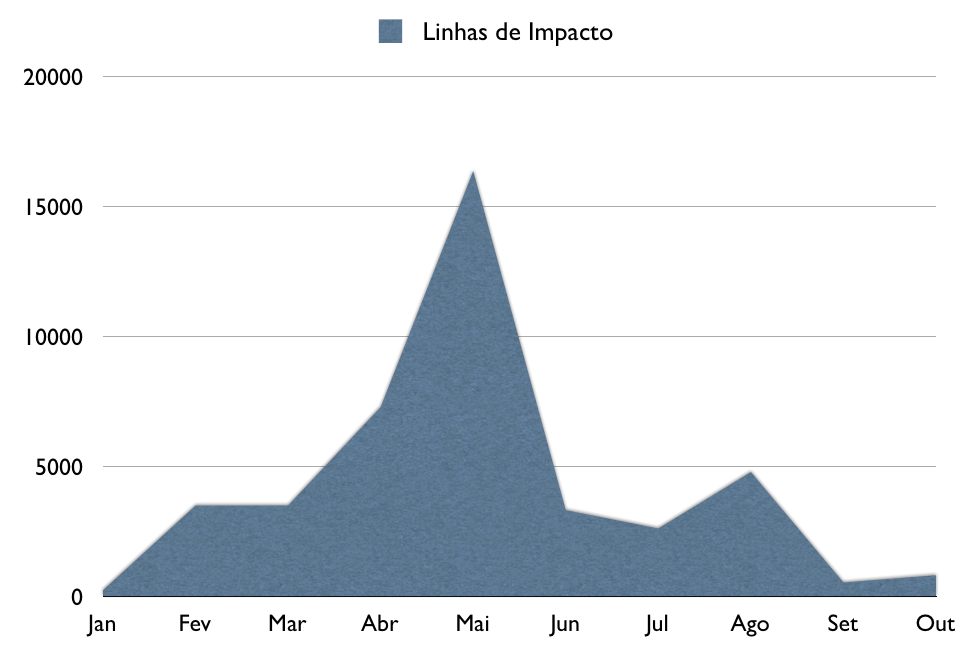
\includegraphics[width=110mm]{images/impacto.png}
  }
  \caption{Linhas de impacto - GitHub}\label{figura:github}
\end{figure}

Esses dados foram coletados do gráfico de impacto do GitHub e as divisões de linhas por desenvolvedor foram removidas porque, como a equipe adota programação pareada na maioria do tempo, as divisões não necessariamente representam a participação única de cada desenvolvedor no projeto.

Nota-se, dessa imagem, um pico de linhas de código enviadas ao repositório no mês de maio, mês seguinte a quando passou-se a gerenciar o próprio \calopsita{} usando a parte que já estava pronta do projeto. Contudo, houve trabalho de janeiro até o momento atual, com uma considerável queda em setembro para que focássemos nessa monografia.

Esse fenômeno é bastante natural: quando começa-se a usar um sistema novo, encontra-se diversos problemas e pontos de melhoria. A pressa para resolver os problemas mais impeditivos demandou um esforço maior da equipe.

\subsection{Gerenciamento do projeto}

Por tratar-se de um projeto de médio porte, seria indicado optar por alguma metodologia de gerenciamento de \software{}. Métodos tradicionais nem sequer foram considerados. Há algumas razões para isso.

Primeiramente porque, buscando informações históricas sobre o modelo \textit{Waterfall}, descobriu-se que mesmo o artigo~\cite{waterfall} que primeiro descreveu o modelo avisava que sua implementação é quase utópica e propensa a falhas.

\begin{quote}
\textit{``I believe in this concept, but the implementation described above is risky and invites failure.'}'
\end{quote}

Mais do que isso, o autor, já em 1970, sugeria que o desenvolvimento iterativo é mais apropriado para o desenvolvimento de projetos de \software{}. Isso apenas aumenta a consternação com relação ao que é ensinado em universidades ao redor do mundo e se vê no mercado de trabalho ainda hoje -- diversas empresas que clamam usar RUP~\cite{rup} ignoram sua parte mais importante, o desenvolvimento iterativo.

Em segundo lugar, métodos tradicionais prezam pelo conhecido \textit{``Big Design Up Front'}', isto é, em planejar toda a arquitetura de um sistema antes de começar a produzí-lo e manter esse \textit{design} até o produto final surgir. Essa ideia pressupõe que, de início, se saiba tudo o que será necessário do sistema e que essas necessidades não mudem. A experiência mostra que, na produção de \software{}, o padrão é não conhecer de antemão o que se precisa e as necessidades mudarem com o tempo~\cite{change}.

De fato, verificou-se a verdade nessa afirmação quando, no início do projeto, os clientes queriam um papel Administrador do Sistema no \calopsita{} que restringiria partes do sistema que podem ser editados por cada tipo de usuário. Essa funcionalidade, assim como diversas outras, acabou não sendo implementada por se mostrar desnecessária.

Finalmente, tanto os desenvolvedores quanto os clientes do \calopsita{} valorizam o \textit{feedback} rápido e atribuem a isso muitos projetos bem-sucedidos. Os clientes têm seus trabalhos de mestrado relacionados com métodos ágeis e anos de experiência nessas metodologias. Os desenvolvedores trabalham diariamente com Scrum~\cite{scrum} e XP~\cite{xp} e possuem certificações pela Scrum Alliance~\footnote{http://www.scrumalliance.org/}. 

A equipe, como um todo, acredita que as metodologias ágeis são uma resposta ao modo engessado com que métodos tradicionais tratam a produção de \software{} e que, aplicando os valores descritos no Manifesto Ágil~\cite{manifesto}, obtemos produtos de qualidade, que atendem às necessidades reais dos clientes e dão satisfação aos desenvolvedores.  

\subsection{Abordagem Ágil}

Embora Scrum não tenha sido usado para desenvolver o \calopsita{}, utilizamos alguns métodos e ferramentas típicos desse
\textit{framework} e de XP que melhor funcionavam para o time. O uso de metodologias e \textit{frameworks} são excelentes para
times e pessoas em migração das formas tradicionais, mas seu uso não se mostrou necessário no time do \calopsita{}. Todos,
clientes e desenvolvedores, têm grande experiência com métodos ágeis e, dessa forma, optou-se por simplesmente seguir os
preceitos ágeis e adaptar os métodos que ajudassem mais a cada etapa. 

\subsubsection*{Kanban~\cite{kanban}}

Como, durante a maior parte do desenvolvimento, os programadores trabalhavam no mesmo espaço físico, pôde-se adotar um quadro branco com \textit{kanban}, uma forma de organização de tarefas bastante difundida na área de Administração que foi portada para \software{} mais recentemente. A figura \ref{figura:kanban} mostra o quadro branco do Calopsita, com o \textit{kanban} à esquerda, visão, anotações e as \textit{personas} à direita -- essas últimas, serão explicadas mais adiante nessa seção.

\begin{figure}[H]
  \centering
  \fbox{
    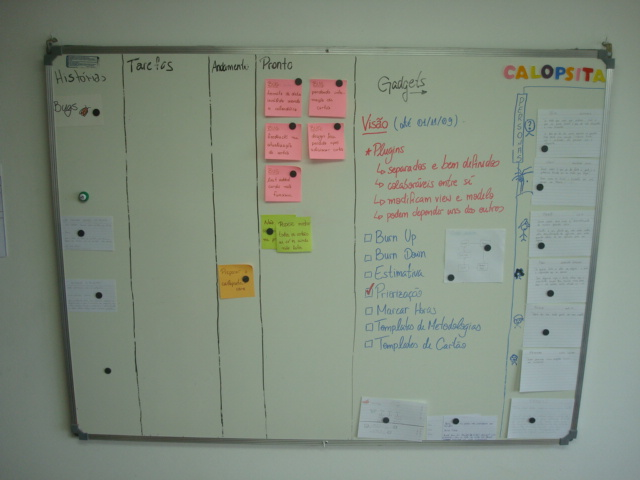
\includegraphics[width=110mm]{images/calopsita-kanban.png}
  }
  \caption{Kanban do \calopsita{}}\label{figura:kanban}
\end{figure}

O quadro branco é uma forma bastante eficiente de comunicação -- basta olhar para ele para entender, de imediato, o que há para ser feito, o que já está pronto e quais tarefas estão em andamento. Além disso, nosso quadro conta com a \textbf{Visão do Projeto}, isto é, a meta maior para o projeto, onde queremos chegar.

\subsubsection*{Integração Contínua}

Para manter o código funcional a cada mudança, utilizou-se, desde o começo do projeto, um servidor de integração contínua~\cite{ci}, o CruiseControl.rb~\footnote{http://cruisecontrolrb.thoughtworks.com/}. Esse servidor é capaz de consultar o repositório de código de tempos em tempos verificando por mudanças no código. Uma vez detectada alguma alteração, ele baixa o novo código, compila e roda seus testes de forma automática. 

Se durante esse processo qualquer um dos testes falhar, um email é disparado para toda a equipe, garantido que o bug introduzido seja corrigido o mais rapidamente possível. Por outro lado, se todos os testes forem executados com sucesso, um \textit{deploy} é feito de forma automática em um servidor de homologação. Isso permite que todos os envolvidos consigam acompanhar e testar, em tempo real, tudo que está sendo implementado. A figura \ref{figura:cruisecontrol} mostra resultados do processo no final de outubro de 2009.

\begin{figure}[H]
  \label{figura:cruisecontrol}
  \centering
  \fbox{
    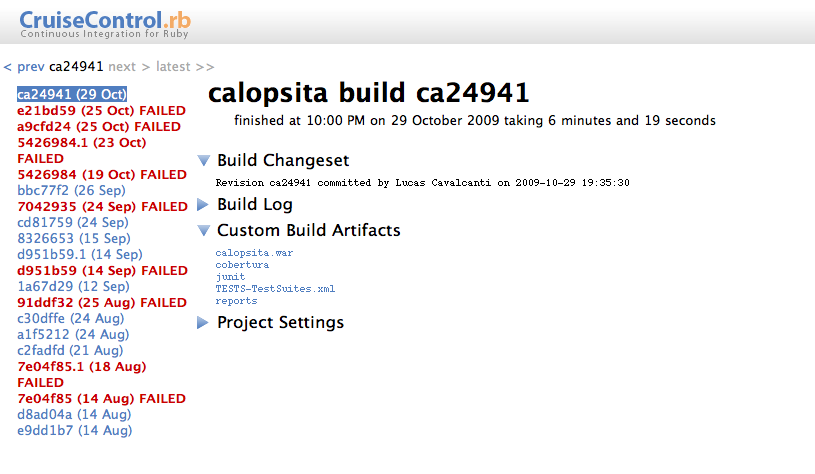
\includegraphics[width=110mm]{images/cruisecontrol-calopsita.png}
  }
  \caption{Cruisecontrol.rb do \calopsita{}}
\end{figure}

\subsubsection*{Pareamento e refatoração}

A qualidade do código, tanto em aspectos de legibilidade quanto em arquitetura, é assegurada por discussões técnicas na lista do projeto, por discussões com profissionais da Caelum e pelo uso extensivo de programação em pares. As vantagens da programação em pares~\cite{pair}, contudo, vão além da manutenção da qualidade de código -- atribuímos a essa prática o nivelamento do conhecimento não apenas sobre o código do Calopsita, mas também sobre os conceitos aplicados em diversas partes do sistema.

Outro fator que colaborou bastante na qualidade do código é a cultura de refatorações que a equipe adota. A regra é que, sempre que se encontra código que poderia ser melhor, melhora-se ele. Isso faz com que o código se mantenha sempre atual e o melhor possível na visão da equipe de desenvolvimento.

\subsubsection*{Interação com clientes}

Para manter o foco do projeto no que era mais valioso para o cliente a cada momento, a interação com esses foi fundamental para o bom andamento do projeto. Houve reuniões semanais ou quinzenais durante todo o ano, onde os clientes testavam o \calopsita{} ambiente de homologação, aprovavam tarefas,  repriorizavam os cartões de funcionalidades e definiam uma meta para a iteração seguinte. 

Com a estabilização do \calopsita{}, diversos projetos da Caelum também começaram a usar o sistema para gerência dos ítens por fazer e iterações. Assim, passamos a ter mais clientes e, portanto, mais pedidos de funcionalidades e correções. Nesse momento, usar o próprio \calopsita{} para auxiliar em seu desenvolvimento se mostrou bastante conveniente: os clientes colocavam seus pedidos no sistema e priorizavam seus cartões.

\subsubsection*{Personas}

Trabalhando com diversos clientes traz um aumento considerável na complexidade de comunicação entre as partes envolvidas no projeto. Tanto a comunicação entre clientes diferentes quanto com a equipe de desenvolvimento foi facilitada com o uso de \textit{Personas}. Os pedidos eram feitos em nome de um personagem cujos valores eram conhecidos pela equipe e pelos clientes. 

Por exemplo, a \textit{persona} \textit{Fabs} representa um usuário do sistema que é um tanto distraído e quer que o sistema não tenha ambiguidades que possam confundí-lo. Com essa descrição, todos sabem que essa persona representa a preocupação com usabilidade e interação homem-computador. Um cartão desse personagem, tirado do \textit{backlog} do \calopsita{}, pode ser visto a seguir, no cartão \ref{tabela:fabs}.

\begin{figure}[H]
  \label{tabela:fabs}
  \begin{tabular}{|p{10cm}|}
    \hline
    Para não me confundir sobre qual cartão eu peguei \\
    Como Fabs \\
    Quero que os cartões na priorização e na iteração mantenham a mesma forma quando são arrastados. \\
    \hline
  \end{tabular}
\end{figure}

A lista e descrições das \textit{personas} usadas na construção do \calopsita{} podem ser encontradas no Apêndice~\ref{app:personas}.

\newpage

\section{Código}

Todo o código do \calopsita{} está hospedado no GitHub, onde podem ser visualizados todo o histórico e atividades realizados no projeto desde sua concepção.

Antes de iniciar o desenvolvimento do \calopsita{}, foi discutido quais seriam as escolhas de linguagens e \textit{frameworks} a serem utilizados. As opções se reduziram a duas: Ruby on Rails ou Java com VRaptor. Como a maioria da equipe tinha mais familiaridade com Java do que com Ruby, a escolha foi pelo Java com VRaptor. Durante o desenvolvimento foram usadas diversos conceitos e boas práticas de desenvolvimento de \software{}, como explicado a seguir.


\subsection{DDD}

A sigla DDD significa \textit{Domain Driven Design}~\cite{ddd}, ou seja, Projeto Orientado ao Domínio. A principal idéia por trás desse conceito é que os clientes e os desenvolvedores falem na mesma linguagem: a linguagem específica de domínio (DSL -- \textit{Domain Specific Language}).

Na forma tradicional de desenvolvimento de software há dois lados claros e quase que opositores no que diz respeito às pessoas envolvidas: o lado do négocio, onde ficam os clientes e gerentes do projeto, e o lado técnico, onde ficam os arquitetos e desenvolvedores. Os clientes e gerentes tendem a conversar usando termos totalmente voltados à realidade de quem vai usar o \software{}, enquanto os arquitetos e desenvolvedores tendem a conversar usando termos técnicos. 

O resultado disso é que os técnicos não entendem completamente os termos do negócio e clientes não entendem quase nada sobre os termos técnicos. Isso cria um impasse e um desconforto quando é necessário fazer uma reunião entre todos os envolvidos no projeto.

Uma saída para resolver esse impasse é combinar uma linguagem ubíqua (\textit{Ubiquitous Language}), isto é, uma linguagem que todos os envolvidos no projeto conhecem. Dessa forma, clientes, usuários, gerentes, desenvolvedores e arquitetos usarão sempre os mesmos termos para descrever o sistema. Os especialistas no negócio devem definir e explicar os termos mais relevantes para os técnicos, que devem usá-los na arquitetura e no desenvolvimento do sistema. Da mesma forma, o pessoal técnico deve explicar os termos mais importantes da arquitetura do sistema para os especialistas no negócio.

No \calopsita{} o domínio são métodos ágeis, então foram definidos os seguintes termos para a linguagem ubíqua:

\begin{itemize}
	\item{\textbf{Projeto (\textit{Project})} - um projeto gerenciado por uma equipe ágil;}
	\item{\textbf{Iteração (\textit{Iteration})} - uma unidade de tempo que representa um ciclo iterativo do método ágil usado;}
	\item{\textbf{Cartão (\textit{Card})} - uma unidade de trabalho, que pode ser uma funcionalidade, uma tarefa, uma história, ou qualquer unidade que represente o que precisa ser desenvolvido;}
	\item{\textbf{\textit{Gadget}} - algo que adiciona informações ao cartão;}
	\item{\textbf{\textit{Plugin}} - uma funcionalidade ou conjunto de funcionalidades que pode ser instalada no sistema.}
\end{itemize}

Toda a arquitetura do sistema se baseia nesses termos e na interação entre eles. Desse modo, a comunicação entre desenvolvedores e clientes acontece sem grandes problemas.

\subsection{BDD e expressividade} 
\label{bdd}

BDD~\cite{bdd}, \textit{Behavior Driven Development}, é, não uma ferramenta, mas uma forma de pensar na sua aplicação. Segundo ela, pensa-se primeiro no comportamento esperado do \software{} e depois no código que será produzido. A recente adoção dessa forma de pensamento tem se mostrado bastante positiva na redução do acoplamento e na expressividade do código.

Desde o começo, decidiu-se adotar boas práticas de desenvolvimento como o uso de \textit{Behavior Driven Development}, refatoração constante e programação em pares. Principalmente, para usar BDD, buscou-se ferramentas que ajudassem a escrever testes mais expressivos e legíveis. 

No mundo do \textit{Ruby on Rails} essa prática já está bastante difundida e, portanto, existem várias ferramentas de teste como o RSpec~\footnote{http://rspec.info/} e o Cucumber~\footnote{http://cukes.info/} que implementam BDD. O dinamismo da linguagem ajuda, possibilitando a escrita de DSLs (\textit{Domain Specific Languages}) e interfaces fluentes~\cite{dsl} de uma maneira bastante direta. 

Em Java, a tendência do uso de BDD ainda não é forte e não existem ferramentas avançadas. Além disso, Java é uma linguagem estática e burocrática, o que torna o desenvolvimento de tais ferramentas muito mais difícil. 

Apesar das limitações impostas pela escolha da linguagem, as vantagens de usar BDD compensavam as dificuldades. Dessa forma, foram pesquisadas as seguintes alternativas:

\begin{itemize}
	\item{\textbf{JBehave}~\footnote{http://jbehave.org/} -- funciona associando um arquivo de texto a um código Java. No arquivo texto, fica a descrição da funcionalidade, tal como seria escrita num cartão de história;}
	\item{\textbf{Cucumber $+$ JRuby}~\footnote{http://jruby.org/} -- tal qual a opção anterior, associa texto a código. Faz isso de uma forma mais eficiente e elegante do que o JBehave, mas é uma solução para Ruby. Precisa usar JRuby para integrar código Java aos testes;}
	\item{\textbf{JUnit} -- a ferramenta padrão para testes automatizados em Java. Não tem nenhuma preparação para BDD, então seria apenas instrumental e se somaria à determinação da equipe por escrever testes legíveis e expressivos.}
\end{itemize}

O JBehave foi descartado por causa da sua sintaxe pouco produtiva, do uso extensivo de herança e de algumas limitações, como a impossibilidade de compartilhar passos (associações entre código Java e etapas da funcionalidade) entre casos de uso.

Cucumber e JRuby foram descartados por causa da complexidade da integração e por causa da mistura de linguagens -- o \calopsita{} é um projeto \opensource{} e a mistura de linguagens poderia afastar eventuais colaboradores.

A última opção foi escolhida por ser mais simples e permitir criar uma nova forma de desenvolver testes em Java. A solução para testes foi publicada no \textit{blog} da Caelum~\footnote{http://blog.caelum.com.br/2009/02/28/behavior-driven-development-com-junit/} e é uma arquitetura de testes que possibilita a escrita de testes de aceitação, em Java, quase em linguagem natural. 

Inspirados no Cucumber, algumas convenções semânticas foram criadas para aumentar a legibilidade, de acordo com suas responsabilidades:

\begin{itemize}
	\item{\texttt{GivenContexts given} -- objeto que vai preparar o contexto inicial do teste em questão. Ex: Entrar em uma página, inserir determinados objetos no banco, logar-se com um dado usuário, etc;}
	\item{\texttt{WhenActions when} -- objeto que vai executar as ações do teste em si, utilizando o contexto definido pelo objeto \texttt{given}. Ex: Preencher um formulário, clicar no botão Enviar, selecionar um item em alguma caixa de opções, etc;}
	\item{\texttt{ThenAsserts then} -- objeto que verifica se o resultado das ações executadas é o esperado. É a parte mais importante do teste. Ex: O usuário está logado? Apareceu a mensagem ``Inserido com sucesso''? Deu erro de validação?}
\end{itemize}

Este é um exemplo de teste escrito nessa arquitetura, retirado do código do \calopsita{}:

\begin{lstlisting}
/**
 * In order to plan what has to be done
 * As a project client
 * I want to create and edit cards (with name and description)
 *
 */
public class CreateACardStory extends DefaultStory {

	@Test
	public void cardCreation() throws Exception {
		given.thereIsAnUserNamed("David").and()
			.thereIsAProjectNamed("Papyrus").ownedBy("David").and()
			.iAmLoggedInAs("David");

		when.iOpenProjectPageOf("Papyrus").and()
		    .iOpenCardsPage().and()
			.iAddTheCard("Incidents")
				.withDescription("create and update an incident").and()
			.iOpenCardsPage();
		then.theCard("Incidents").appearsOnList();
	}
}
\end{lstlisting}

Repare que se os ruídos sintáticos pudessem ser removidos, o mesmo código seria lido com:

\begin{verbatim}
In order to plan what has to be done
As a project client
I want to create and edit cards (with name and description)

Create a card story:

card creation:
	
	given there is an user named "David" and
		there is a project named "Papyrus" owned by "David" and
		i am logged in as "David"

	when I open project page of "Papyrus" and
		I open cards page and
		I add the card "Incidents" 
			with description "create and update an incident" and
		I open cards page
			
	then the card "Incidents" appears on list
\end{verbatim}

Isso é bastante próximo da linguagem natural, em inglês, e possibilita a leitura fácil até para leigos.

Essa arquitetura de testes foi adotada apenas para testes de aceitação, que eram escritos a cada solicitação de funcionalidade. Para os testes unitários, a solução para aumentar a legibilidade foi  apenas usar refatoração, em especial a \textit{Extract Method}~\cite{refactoring}, para criar a mesma sensação, apesar de conter um pouco mais de ruídos sintáticos do Java. Um exemplo de teste unitário, retirado do código do \calopsita{}:

\begin{lstlisting}
public class IterationTest {
	@Test
	public void addingACardToAnIteration() throws Exception {
		Iteration iteration = givenAnIteration();
		Card card = givenACard();

		shouldUpdateTheCard(card);

		whenIAddTheCardToIteration(card, iteration);

		assertThat(card.getIteration(), is(iteration));
		mockery.assertIsSatisfied();
	}
}
\end{lstlisting}

Novamente, removendo a burocracia da linguagem de programação, obtemos o seguinte resultado.

\begin{verbatim}
Adding a card to an iteration
	given an iteration
	given a card

	should update the card

	when I add the card to iteration

	assert that the card's iteration is the given iteration
\end{verbatim}

Dessa forma, a manutenção dos testes fica muito fácil e pode ser feita facilmente por qualquer pessoa, já que o teste deixa bem claro que está fazendo.

\subsection{SeleniumDSL e testes de aceitação}

No processo de desenvolvimento do \calopsita{}, foram criados testes de aceitação para cada funcionalidade requisitada pelos clientes do projeto. Esses testes são feitos a partir dos cartões escritos pelos clientes e são usados para validar se a funcionalidade está pronta. 

Testes de aceitação simulam a interação do usuário com o sistema, executando passos como preencher formulários, clicar em botões, arrastar e soltar componentes. Esses testes de aceitação foram escritos em duas etapas: a primeira, em linguagem praticamente natural como visto na seção \ref{bdd}, e a infraestrutura para que essa primeira funcione corretamente, isto é, a implementação real das ações do teste.

Para executar os testes, precisamos ter a aplicação rodando em um servidor e, então, simular a interação de um usuário com o sistema. Esta, pode ser simulada de duas formas:

\begin{itemize}
	\item{Abrindo um navegador, como o Firefox ou o Safari, e simulando as ações do usuário via javascript. A principal	ferramenta para isso é o Selenium~\footnote{http://seleniumhq.org/}. 

Uma das vantagens dessa abordagem é que se pode acompanhar os passos do teste visualmente, facilitando a identificação de erros no teste. Entre as desvantagens, salta à vista a demora da execução dos testes, pois envolve a criação de novos e grandes processos no sistema operacional: o navegador precisa ser aberto e o Selenium requer uma instância de seu servidor rodando;}
	\item{Criar as páginas da aplição em memória. A principal ferramenta para isso, em Java, é o HtmlUnit~\footnote{http://htmlunit.sourceforge.net/}. 

Uma das vantagens é que, por fazer tudo em memória, a execução dos testes é bem mais rápida. Mas, exatamente por ser em memória, não é possível visualizar a execução do teste, o que torna a depuração mais complicada.}
\end{itemize}

O \calopsita{} começou usando o Selenium para os seus testes de aceitação. Mas a interface de uso do Selenium é difícil de utilizar e não é orientada a objetos: uma única interface com quase 150 métodos que contêm todas as ações existentes para uma página. Por causa disso, muitos projetos surgiram para tornar essa interface mais agradável de trabalhar. Um desses projetos é o SeleniumDSL~\footnote{http://github.com/caelum/selenium-dsl}, que é um projeto \opensource{} desenvolvido por pessoas da Caelum, inclusive os membros do \calopsita{}. O Selenium DSL é uma Fachada (\textit{Façade})~\cite{gof} que transforma a interface procedural numa interface fluente~\cite{dsl} e orientada a objetos.

Para usar o Selenium, precisamos de um servidor Selenium rodando, que vai tratar as requisições dos testes, abrir navegadores e executar comandos. Isso causa certos problemas para configurá-lo em um processo de integração contínua~\cite{ci}, pois é preciso garantir que o servidor esteja rodando antes de executar os testes, e é necessário ter um servidor gráfico rodando para que os navegadores possam ser abertos. Por esse motivo, resolveu-se migrar os testes para o HtmlUnit, que não precisa de recursos externos para executar.

Como a API SeleniumDSL é toda baseada em interfaces, foi criada, usando o \calopsita{} como base, uma implementação para HtmlUnit, transformando, dessa forma, o SeleniumDSL num Adaptador(\textit{Adapter})~\cite{gof}: não foi preciso mudar a implementação dos testes no \calopsita{}, tudo continuou funcionando quando a implementação do SeleniumDSL foi trocada. 

Além disso, o SeleniumDSL permite trocar da implementação em Selenium para a em HtmlUnit mudando apenas uma linha de código. Por isso, criamos uma Fábrica(\textit{Factory})~\cite{gof} que decide qual das implementações do SeleniumDSL vai ser usada, fazendo com que aproveitássemos as vantagens das duas formas de criar testes para a web: usar o Selenium durante o desenvolvimento dos testes, para facilitar a depuração, e usar o HtmlUnit para rodar os testes no ambiente de integração contínua, para maior rapidez nos testes e simplicidade. Essa implementação de HtmlUnit para SeleniumDSL foi assunto de uma palestra num evento interno da Caelum~\footnote{http://www.youtube.com/watch?v=5oFlh\_Ka65U\&feature=related}.

\subsection{REST}

O termo REST (\textit{Representational State Transfer}) foi cunhado por Roy Thomas Fielding em sua tese de doutorado~\cite{rest-roy}, onde ele descreve as idéias que levaram à criação do protocolo HTTP.

É um modelo arquitetural para sistemas distribuídos e a proposta central é que existe, no protocolo HTTP, um conjunto fixo de operações permitidas (verbos) e diversas aplicações que se comunicam aplicando este conjunto fixo de operações em recursos existentes. As aplicações podem, ainda, solicitar diversas representações destes recursos.

A web é o maior exemplo de uso de uma arquitetura REST, onde os verbos são as operações disponíveis no protocolo (GET, POST, PUT, DELETE, HEADER, TRACE, OPTIONS), os recursos são identificados pelas URIs~\footnote{URI: Uniform Resource Identifier} e as representações podem ser definidas através de \textit{Mime Types}~\cite{mimetypes}.

Ao desenhar aplicações REST, pensa-se nos recursos a serem disponibilizados pela aplicação e em seus formatos, em vez de pensar nas operações. Isso é facilmente reconhecido por URIs bastante expressivas. No \calopsita{}, as idéias de REST são utilizadas. Por exemplo, uma mesma URI de iteração (recurso) é capaz de adicionar, mostrar, atualizar e remover uma iteração.

\begin{verbatim}
 GET /projects/5/iterations => lista as iterações do projeto 
                               de id 5
 POST /projects/5/iterations => adiciona uma iteração ao 
                                projeto de id 5
 GET /projects/5/iterations/10 => visualiza a iteração de id 
                                  10 do projeto de id 5
 PUT /projects/5/iterations/10 => atualiza a iteração de id 
                                  10 do projeto de id 5
 DELETE /projects/5/iterations/10 => remove a iteração de id 
                                     10 do projeto de id 5
\end{verbatim}

O recurso \texttt{/project/5/iterations} responde adicionando uma iteração quando é chamado via \texttt{POST} e listando todas as iterações quando chamado via \texttt{GET}. As outras operações, que poderiam ser acessadas por outros métodos HTTP, por exemplo, \texttt{DELETE} removendo todas as iterações do projeto e \texttt{PUT} substituindo a lista de iterações do projeto, não fazem sentido no contexto do \calopsita{}, então não foram implementadas.

\subsection{VRaptor e Injeção de Dependências}

Ao desenvolver aplicações web, tem-se duas escolhas: orientação a componentes ou a ações. Aplicações orientadas a componentes na Web costumam dar uma sensação de artificialidade. Isso porque a Web não possui suporte nativo a esse tipo de abordagem. Além disso, os \textit{frameworks} orientados a componente existentes em Java não possuem boa testabilidade e atrapalham a produtividade. 

A decisão de desenvolver o \calopsita{} orientado a ações vem da propensão da arquitetura da web a lidar com ações curtas e pontuais. Dentre os \textit{frameworks} orientados a ações disponíveis para Java, o VRaptor~\footnote{http://vraptor.caelum.com.br} foi eleito, tanto pela maior familiaridade da equipe, quanto por esse \textit{framework} se mostrar mais produtivo e simples que os outros.

Começamos a desenvolver o \calopsita{} com o VRaptor na versão 2.6, a mais atual na época. Paralelamente, a versão nova do VRaptor, a 3.0, começou a ser desenvolvida. Por volta de julho, já havia uma versão alfa funcional. Então, o \calopsita{} foi migrado para o VRaptor 3, já que ele trazia idéias melhores e boas práticas, muitas provenientes do \textit{Ruby on Rails}. 

Além disso, vislumbrou-se a possibilidade de o \calopsita{} auxiliar no desenvolvimento do VRaptor 3, como pode ser visto no Apêndice~\ref{app:vraptor}. Ambos são projetos \opensource{} e possuem desenvolvedores em comum. Graças a relação entre os projetos, tanto o \calopsita{} quanto o VRaptor 3 amadureceram e cresceram.

O VRaptor 3.0 possibilita o desenvolvimento de aplicações RESTful~\cite{rest} e o uso massivo de injeção de dependências~\cite{di}. O uso de uma interface web RESTful traz várias vantagens para uma aplicação web. Usando os verbos HTTP da forma recomendada na concepção do protocolo, pode-se aproveitar a semântica da web para uma aplicação. Além disso, o uso da arquitetura REST permite aproveitar recursos dos servidores, como caching. Também, a aplicação se torna automaticamente um \textit{web-service}, cada página representando um recurso, facilitando a integração com outros sistemas.

Em julho, o \calopsita{} foi totalmente migrado para VRaptor 3, aumentando sensivelmente a produtividade no desenvolvimento. Nessa época, o VRaptor ainda não tinha uma versão estável, mas a maneira com o que ele foi feito possibilitava a fácil personalização e resolução dos problemas que existiam nele. A versão final só saiu no começo de outubro, mas entre julho e outubro o \calopsita{} auxiliou no desenvolvimento e teste das versões \textit{beta} do VRaptor 3.

Usar injeção de dependências reduz grande parte dos códigos de infraestrutura e elimina a necessidade de instanciação de objetos em diversos métodos de uma mesma classe. Dessa forma, faz com que a aplicação fique naturalmente mais testável e com menor acoplamento. Isso, aliado a \textit{Factory Methods}~\cite{gof} e o uso de interfaces ao invés de implementações~\cite{effective}, fez com que as classes do \calopsita{} ficassem fáceis de testar unitariamente, possibilitando uma cobertura por testes de mais de 90\%.

\subsection{\textit{ActiveRecord}}

O padrão \textit{Active Record}~\cite{fowler} se tornou conhecido após o surgimento do Ruby on Rails~\footnote{http://rubyonrails.org}, que o usa para fazer a persistência dos dados. A idéia é que os próprios objetos sejam responsáveis por sua persistência, em vez de haver classes especializadas em salvar objetos do modelo no banco de dados. Essa segunda forma é denominada \textit{Data Mapper}~\cite{fowler}.

Em Java, o padrão \textit{Data Mapper} é, de longe, o mais utilizado, já que há ótimas ferramentas de mapeamento objeto-relacional (ORM)~\cite{orm}, como o Hibernate, para auxiliar na questão da persistência. Faz parte da cultura da própria linguagem o uso extensivo do Hibernate~\footnote{http://hibernate.org} e de DAOs (\textit{Data Access Object})~\cite{dao}.

Os DAOs são objetos que formam uma camada de abstração e tornam o acesso ao banco de dados mais simples e independente da forma de persistência dos dados. Parece bastante elegante, mas, usando esse padrão de projeto, é usual encontrar o seguinte exemplo de método, numa classe de acesso a dados:

\begin{lstlisting}
public List<Cartao> listaCartoesDoProjeto(Projeto projeto) {...}
\end{lstlisting}

Esse código não está orientado a objetos, embora receba e devolva objetos -- é uma classe procedural, que pode ser chamada de qualquer lugar e não tem relação direta com a classe de modelo \texttt{Projeto}. Esse mesmo código poderia ser escrito como:

\begin{lstlisting}
public class Projeto {
	//...
	List<Cartao> getCartoes() {...}
}
\end{lstlisting}

Esse segundo exemplo é um trecho bem mais orientado a objetos -- é responsabilidade do projeto conhecer seus cartões, não de uma classe terceirizada. O Hibernate já possibilita esse tipo de código quando se tem relacionamentos de chave estrangeira configurados no modelo, através de \textit{Proxies}~\cite{gof}. No modo padrão de execução dessa biblioteca, ao fazer uma consulta ao banco de dados, os dados não são diretamente carregados. Apenas na primeira vez que um método do objeto carregado é acessado, seus dados são trazidos do banco. 

Nem sempre, contudo, tem-se um relacionamento direto. Suponha, por exemplo, que é necessário obter apenas os cartões ativos. Nesse caso é preciso realizar uma consulta ao banco de dados, e para criar um método como \texttt{getCartoesAtivos} o banco de dados tem que estar acessível a partir do modelo e, assim, é necessário injetá-lo. Em Ruby, isso é possível através de \textit{mixins}~\footnote{http://www.rubycentral.com/pickaxe/tut\_modules.html}, que interpretam invocações a métodos que não existem no modelo e traduzem-nas para consultas ao banco de dados. Em Java, é obrigatório declarar explicitamente os métodos, logo não é possível usar a linguagem para interpretar métodos arbitrários.

A saída foi adotar o padrão \textit{Repository} do livro Domain Driven Design~\cite{ddd} e usar injeção de dependências para que o modelo receba o seu respectivo repositório de dados. Desse modo, adicionam-se métodos que apenas delegam o trabalho para o repositório, a classe que vai fazer a consulta ao banco de fato.

Injetar dependências em modelos não é uma tarefa trivial, porque objetos de modelos são criados várias vezes, em diversas condições diferentes. Algumas criações, por exemplo, são feitas pelo Hibernate quando ele efetua listagens. Outras vezes, esses modelos são criados a partir de parâmetros da requisição web.

Quando o \textit{Active Record} começou a ser implementado no \calopsita{}, o VRaptor não suportava esse tipo de injeção de dependências, então o próprio \calopsita{} implementou essa injeção sobrescrevendo alguns componentes do VRaptor. Um pouco antes do VRaptor lançar sua versão final, contudo, surgiu um projeto \opensource{} chamado IOGI~\footnote{http://github.com/rafaeldff/iogi}, que permite criar objetos imutáveis a partir de parâmetros da requisição. Além disso, o IOGI possibilita a injeção de dependências, extinguindo a necessidade de fazer isso no \calopsita{} e diminuindo, novamente, a quantidade de código de infraestrutura existente.

Desse modo, criamos modelos ricos, que encapsulam o seu acesso e representação no banco de dados. Assim os controladores das requisições web não precisam lidar com operações do banco de dados, eles apenas usam a interface do próprio modelo para fazer isso.

\subsection{Arquitetura de plugins}

Para facilitar a contribuição ao projeto, decidiu-se por adotar uma arquitetura de plugins no \calopsita{}. Desse modo existe um núcleo bem definido do sistema e os plugins definem pontos de extensão através dos quais podem adicionar informações e funcionalidades ao sistema.

O núcleo consiste nas seguintes entidades básicas do sistema:

\begin{itemize}
	\item{\textbf{Card} - \textit{Cartões} - representam funcionalidades, etapas de desenvolvimento, tarefas, histórias de usuário etc. São a unidade básica das metodologias ágeis. Em ambientes físicos, são usualmente representados por cartões colados em quadros brancos;}
	\item{\textbf{CardType} - \textit{Tipos de cartão} - adicionam ao cartão uma semântica. Com isso podemos dizer que um cartão \textbf{é uma} tarefa, uma história ou um épico, por exemplo. Com tipos de cartão também pode-se criar \textit{templates} que serão aplicados aos cartões desse tipo, por padrão;}
	\item{\textbf{Iteration} - \textit{Iterações} - representa uma iteração, que é uma unidade de trabalho de metodologias ágeis. Iterações representam um ciclo de trabalho e entrega de funcionalidades;}
	\item{\textbf{Project} - \textit{Projetos} - representa um projeto gerenciado pelo calopsita;}
	\item{\textbf{User} - \textit{Usuários} - representa um usuário do sistema.}
\end{itemize}

Com essas entidades é possível controlar a parte central do sistema. Elas foram escolhidas de forma minimal por serem comuns a qualquer metodologia ágil. 

Mas além delas, há a parte dos \textit{plugins}, que permitem desenvolver as funcionalidades específicas de cada metodologia ou adaptação de metodologia adotada pelo projeto. Os \textit{plugins} são classes que implementam uma interface dos pontos de extensão. Isto é, ao escrever essas classes, o comportamento do sistema é alterado adicionando uma funcionalidade ou simplesmente modificando listagens. Os pontos de extensão existentes são os seguintes:

\begin{itemize}
	\item{\textbf{Gadget} - Com ele você pode adicionar informações e comportamento aos cartões. Por exemplo adicionar tempo estimado de execução e data de início e finalização;}
	\item{\textbf{PluginConfig} - Responsável por integrar o plugin ao sistema, adicionando \textit{links} aos menus;}
	\item{\textbf{Transformer} - Responsável por modificar listagens, adicionando, removendo ou ordenando elementos.}
\end{itemize}

Além disso, se o \textit{plugin} precisar adicionar telas ao sistema, ele precisa implementá-las, usando o VRaptor3 para criar um controlador e as JSPs necessárias. Os pontos de extensão existentes ainda não possibilitam modificar telas já existentes, nem mudar formulários, por exemplo, mas podem ser implementados à medida em que forem necessários. Um pequeno manual sobre como criar um plugin pode ser visto no Apêndice~\ref{app:plugins}.

\subsection{Cartões e subcartões}

Cada cartão no \calopsita{} leva consigo tanto suas informações específicas, como descrição e criador, mas também uma lista de outros cartões. Se a arquitetura do \calopsita{} fosse fixa para tipos de cartões e determinasse que apenas haveriam as categorias ``História'', ``Tarefa'' e ``Bug'', certamente haveria aí uma implementação do padrão de projeto \textit{Composite}~\cite{gof}.

Com a preferência pela flexibilidade, um cartão tem uma lista de cartões e uma lista de \textit{gadgets}. A presença ou ausência de \textit{gadgets} é que caracteriza cada tipo de cartão. Exemplificando, define-se o seguinte conjunto de \textit{gadgets} aos cartões:

\begin{itemize}
	\item{Histórias: têm \textit{gadgets} Priorizável, Planejável e Pontuável;}
	\item{Tarefas: têm o \textit{gadget} de participação do Kanban;}
	\item{\textit{Bugs}: têm \textit{gadgets} Priorizável e Planejável;}
\end{itemize}

Nesse exemplo, na tela de priorização, aparecerão apenas os cartões de Histórias e Bugs. Já no gráfico de \textit{Burn Down}, apenas as Histórias aparecem porque apenas elas contam pontos.

Dessa forma, o \calopsita{} usa \textit{Composite} conceitualmente, apesar da implementação não estar estritamente de acordo com o proposto nos padrões de projeto. Os \textit{gadgets} somados a um cartão poder conter outros cartões, suprem o papel feito pelo polimorfismo daquela descrição e servem à resolução do mesmo problema. 

\newpage

\section{Funcionalidades}

No \calopsita{}, também por sua arquitetura de \textit{plugins}, as funcionalidades estão separadas em duas grandes partes: o núcleo e os \textit{plugins}. A primeira, contém apenas partes diretamente relacionadas com desenvolvimento ágil, no sentido mais amplo e irrestrito do termo -- sem interferência de metodologias, seus métodos e métricas. Essas partes, variáveis de cada projeto ou dependentes de metodologia, são deixadas para os \textit{plugins}, que dão ao sistema uma melhor adaptabilidade.

\subsection{Calopsita \textit{Core}}

As funcionalidades que fazem parte do núcleo do \calopsita{} consistem da criação e administração de usuários, projetos, cartões e iterações. Parece ser um núcleo minimal e essa é a intenção. Também faz parte do núcleo toda a infraestrutura necessária para a integração de um plugin ao sistema.

Essa seção se inicia com a proposta dos cartões, que é um tanto diferente e precisa ser explicada.

\subsubsection*{Cartões}

Diferente de outros sistemas com o mesmo propósito, o \calopsita{} não possui o conceito de histórias, mas apenas de cartões. Isso foi feito pensando em trazer maior grau de personalização para os usuários. Cada cartão pode ter subcartões e o que define a funcionalidade desse cartão é o conjunto de \textit{gadgets} que ele possui. 

A vantagem é que pode-se criar uma hierarquia, tão profunda quanto se desejar, para organizar tudo o que há para ser feito em um projeto. Isso também permite que o projeto possa ser visto no nível de detalhe mais apropriado pra cada envolvido no projeto, seja ele gerente, desenvolvedor ou cliente. 

\begin{figure}[H]
  \centering
  \fbox{
    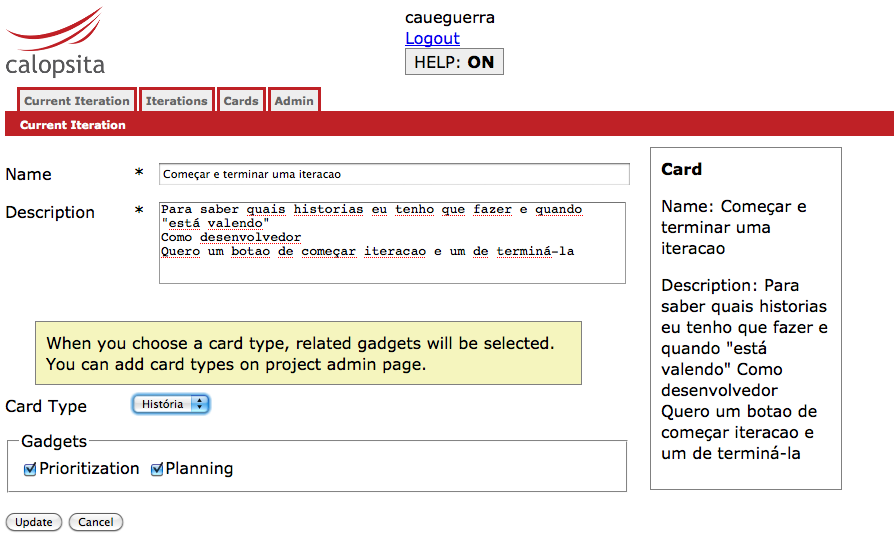
\includegraphics[width=110mm]{images/cartao.png}
  }
  \caption{Cartão}\label{figura:cartao}
\end{figure}

\begin{figure}[H]
  \centering
  \fbox{
    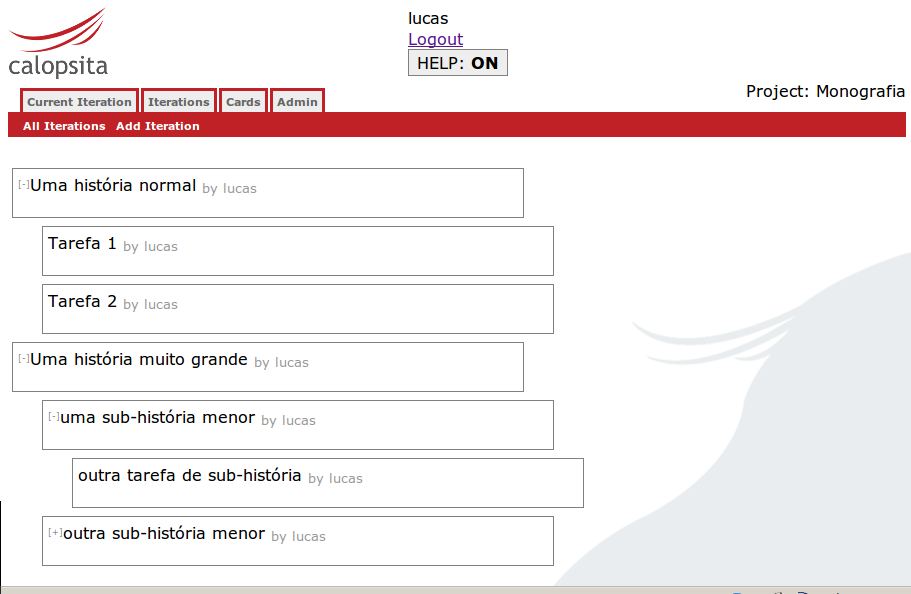
\includegraphics[width=110mm]{images/hierarquia-de-cartoes.png}
  }
  \caption{Cartões mostrados hierarquicamente}\label{figura:hierarquia}
\end{figure}

Já foi dito que usabilidade é uma questão importante para o \calopsita{}. Para determinar hierarquia de cartões foi cogitado utilizar cores diferentes para cartões de mesma grandeza. Preferiu-se, no entanto, usar a indentação mostrada na figura \ref{figura:hierarquia} para manter o sistema acessível para daltônicos.

\subsubsection*{Tipos de Cartões}

Um tipo de cartão é, para o \calopsita{}, um agrupamento de \textit{gadgets} que definem o comportamento de um determinado cartão. Perceba que a noção é puramente semântica, já que os \textit{gadgets} podem ser habilitados e desabilitados individualmente, por cartão.

No exemplo da figura \ref{figura:tipo_cartao}, abaixo, um tipo de cartão denominado ``História'' é criado e, a ele, são associados os \textit{gadgets} ``Priorização'' e ``Planejamento''. Deste momento em diante, sempre que um cartão do tipo ``História'' for criado, ele automaticamente marcará os \textit{gadgets} citados.

Dessa forma, a história criada aparecerá na tela de priorização e poderá ser adicionada a uma iteração -- por ser, respectivamente priorizável e planejável. 

\begin{figure}[H]
  \centering
  \fbox{
    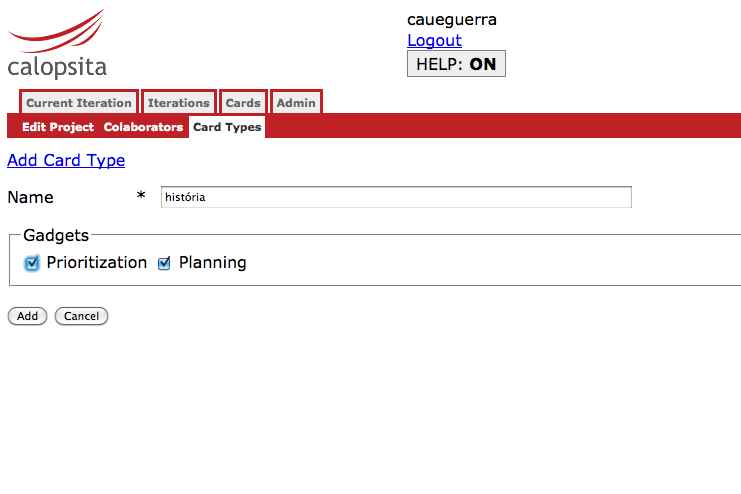
\includegraphics[width=110mm]{images/tipo_cartao.png}
  }
  \caption{Tipos de Cartões}\label{figura:tipo_cartao}
\end{figure}

\subsubsection*{Iterações}

Uma iteração é um ciclo de desenvolvimento ágil. No \calopsita{} é possível criar iterações, editar e removê-las. Na sua criação, é preciso estabelecer uma meta ou um tema da iteração e, além disso, pode-se escolher suas datas de início e fim.

Essas datas são opcionais já que ter ou não datas fechadas depende, exclusivamente, da metodologia adotada pelo time. Em \textit{Scrum}, por exemplo, as datas são pré-fixadas e imutáveis. Já em \textit{XP} preza-se mais pela flexibilidade e uma iteração pode começar ou acabar a qualquer momento.

Um time de \textit{Scrum} que use o \calopsita{} colocaria as datas de antemão e, no dia de início de uma iteração, veria-a começando automaticamente (no menu, ``Iteração atual''). Já um time de \textit{XP} quando quisesse começar uma iteração, clicaria num ícone de \textit{Play} na iteração que deseja começar e num de \textit{Stop} para terminá-la. Se já houvesse datas e, por exemplo, a iteração fosse adiantada alguns dias, o intervalo de tempo entre o início e o fim se manteria -- ambas as datas seriam adiantadas. Veja o exemplo de ícone para iniciar uma iteração futura na figura \ref{figura:play}:

\begin{figure}[H]
  \centering
  \fbox{
    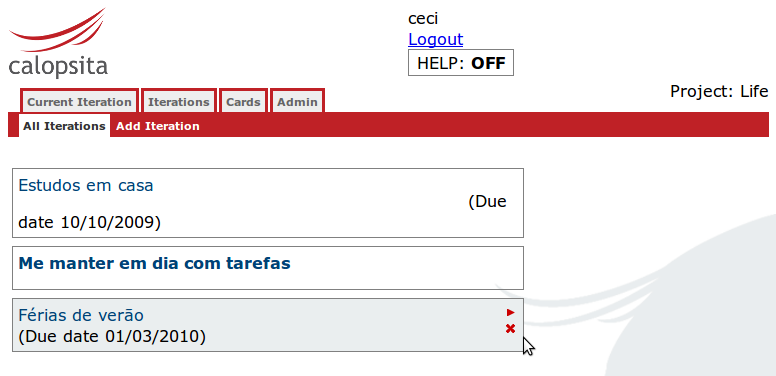
\includegraphics[width=110mm]{images/play_iteracao.png}
  }
  \caption{Adiantar o início de uma iteração}\label{figura:play}
\end{figure}

\subsubsection*{Usuários e projetos}

Por padrão, qualquer usuário pode se cadastrar no sistema. Basta preencher o cadastro com informações pessoais. Igualmente, qualquer usuário logado pode criar projetos.

Num projeto, é possível adicionar colaboradores. Para isso, há uma seção administrativa que permite adicionar um outro usuário ao projeto. Escolhe-se o usuário digitando o \textit{login} dele no campo de seleção ou escolhendo na lista de usuários disponíveis. Essa lista mostra apenas os usuário que ainda não fazem parte do projeto em questão.  

\subsubsection*{Registro de mudanças}

Está previsto para também fazer parte do núcleo do \calopsita{} uma funcionalidade de histórico de mudanças. Assim, será possível coletar informações para gerar gráficos e criar serviços que retornem as últimas modificações feitas, em formato RSS, para que os membros do projeto possam utilizar agregadores de notícias como o \textit{Google Reader} para acompanhar o andamento da iteração.

\subsection{Calopsita Plugins}

Como explicado anteriormente, o \calopsita{} possuí um núcleo com as funcionalidades essenciais e as demais serão fornecidas através de \textit{plugins}. Há, no \textit{backlog} do \calopsita{}, diversos plugins a serem implementados e que já viriam na instalação padrão do \calopsita{}. Segue abaixo uma breve descrição de cada um deles:

\begin{itemize}
	\item{Priorização: permite seja atribuída uma prioridade a um determinado cartão através de uma interface baseada em \textit{drag 'n' drop}. Esse plugin já está implementado;
	
	\begin{figure}[H]
	  \centering
	  \fbox{
	    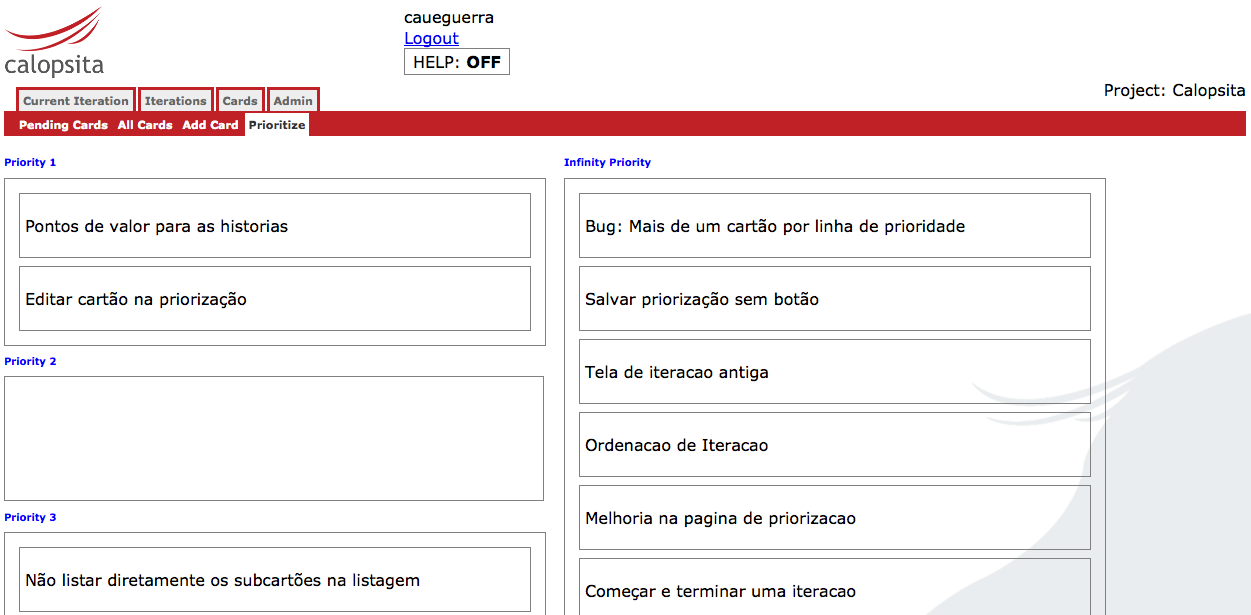
\includegraphics[width=110mm]{images/priorizacao.png}
	  }
	  \caption{Priorizacao}\label{figura:priorizacao}
	\end{figure}
	}
	\item{Planejamento: permite que cartões sejam adicionadas ou removidas de uma determinada iteração. Também baseado em \textit{drag 'n' drop} e já está implementado;
	
	\begin{figure}[H]
	  \centering
	  \fbox{
	    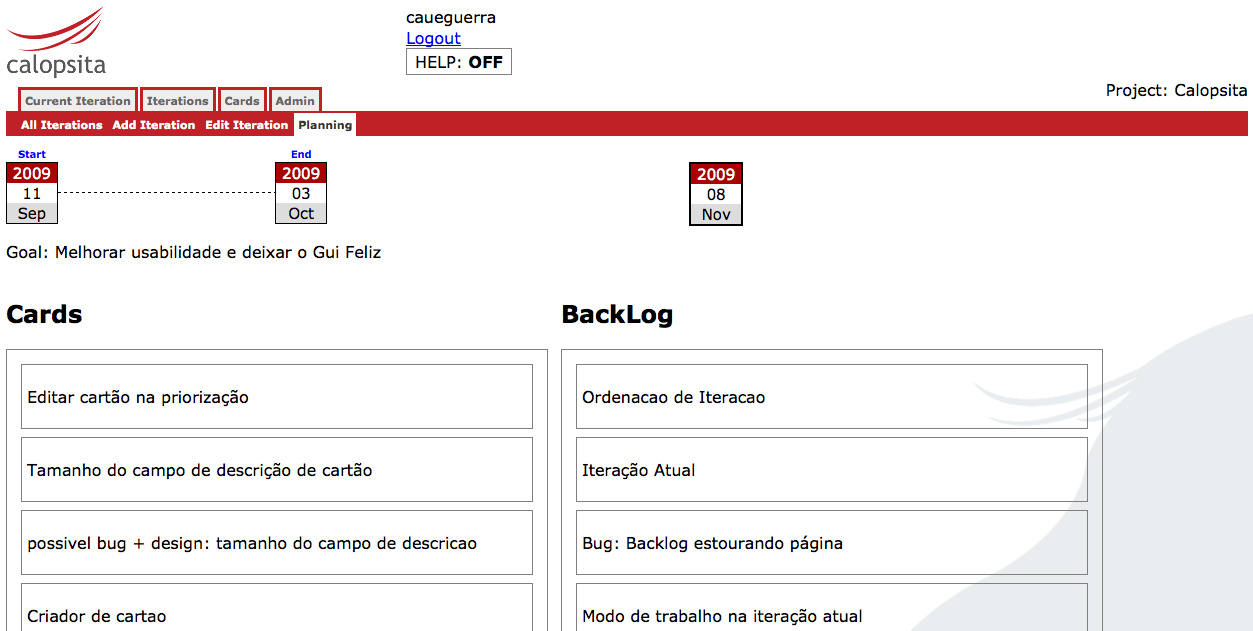
\includegraphics[width=110mm]{images/planejamento.png}
	  }
	  \caption{Planejamento}\label{figura:planejamento}
	\end{figure}
	}
	\item{Gráfico \textit{burn-up}: a idéia desse plugin é que uma nova página contendo o gráfico \textit{burn-up} de uma determinada iteração seja criada. Este gráfico possui uma linha horizontal, que representa a meta a ser atingida. Essa meta é baseada em alguma métrica da iteração: número de cartões, soma da dificuldade dos cartões, etc. Com o passar dos dias da iteração é marcada a evolução da métrica escolhida, de acordo com o número de cartões prontos;}
	\item{Gráfico \textit{burn-down}: a idéia desse plugin é que uma nova página contendo o gráfico \textit{burn-down} de uma determinada iteração sejá criada. Esse gráfico é parecido com o de \textit{burn-up}, mas a evolução se dá pela quantidade de uma métrica que ainda não está pronta. Geralmente possui uma linha decrescente que representa a velocidade estimada;}
	\item{Marcação de horas: esse plugin permitirá que a pessoa que trabalhou na conclusão de determinado cartão possa marcar o número de horas trabalhadas;}
	\item{Estimativas: possibilitará que um cartão tenha sua dificuldade estimada em pontos;}
	\item{Personas: criará uma área especial para a definição de personas. Essas personas poderão ser utilizadas mais facilmente na criação de novos cartões;}
	\item{Integração com GitHub: permitirá que comentários feitos no \textit{commit} do projeto no GitHub consigam mover cartões dentro de uma determinada iteração e mudar seu status.}
	\item{Modelos de metodologias: disponibilizará modelos pré-prontos com tipos de cartão, nomenclaturas e \textit{gadgets} habilitados que são específicos de uma metodologia. Por exemplo um modelo \textit{Scrum} teria os tipos de cartão ``História'', ``Épico'' e ``Tarefa'', a iteração se chamaria ``Sprint'' e teria uma ``Meta'', o \textit{Kanban} com as colunas ``Parado'', ``Em Andamento'', ``Em inspeção'' e ``Pronto'', etc.}
\end{itemize}

\newpage

\section{Visão dos clientes e comparativos}

\subsection{Visão dos clientes}

A fim de obter \textit{feedback} dos clientes quanto às atividades realizadas durante o desenvolvimento desse projeto,
um questionário~(Apêndice~\ref{entrevista}) sobre visão inicial, processo e resultados foi elaborado.

Quanto à visão no início do projeto, a Mari e o Hugo imaginavam um sistema que substituísse o que eles vinham usando atualmente, o \textit{XPlanner}. O foco para os dois era, portanto, oferecer uma solução com melhor usabilidade. Já o Guilherme, imaginava poder substituir o uso de cartões físicos e do quadro branco pelo \calopsita{} -- na Caelum, alguns projetos ocorrem com o time distribuído em suas unidades.

Sobre o processo de desenvolvimento, a Mari e o Hugo gostaram bastante, de uma maneira geral. Algumas críticas foram feitas em relação à distância entre o time e os clientes nos momentos de programação e a dificuldade em saber o que estava pronto antes de o \calopsita{} começar a ser utilizado para o gerenciamento do projeto. Por outro lado, gostaram de poder gerenciar o \calopsita{} usando o próprio \calopsita{} assim que isso foi possível, de terem criado \textit{personas} para a criação de histórias e do \textit{deploy} automatizado, que permitia que eles acompanhassem o trabalho já executado em tempo real. 

Por fim, na questão sobre os resultados obtidos, se mostraram extremamente satisfeitos -- mesmo reconhecendo que o sistema ainda tem muito a melhorar. Disseram que a adoção do \calopsita{} é bastante viável e que, em termos de usabilidade, já supera a ferramenta anterior, como enfatizado pelo Hugo na seguinte frase:

\begin{quote}
``A usabilidade é inquestionável, o \calopsita{} é um projeto que mostra \textbf{claramente} uns 15 anos de avanço em cima do \textit{XPlanner} do ponto de vista da usabilidade.''
\end{quote}

\subsection{Comparativo com outras ferramentas}

Antes de iniciar o desenvolvimento do \calopsita{}, analisou-se outras alternativas de proposta semelhante disponíveis no mercado. Uma análise bem extensa foi feita, tanto de produtos pagos, quanto de gratuitos e \opensource{}. A intenção é descobrir quais os pontos fortes de cada ferramenta e implementá-los no \calopsita{}. 

Embora as ferramentas pagas não sejam exatamente concorrentes, dado o grande investimento que é feito nelas, mostrar que o sistema desenvolvido tem as mesmas ou mais funcionalidades que as alternativas pagas pode fazer com que mais usuários e colaboradores sejam atraídos.

\begin{itemize}
\item{\textbf{Scrumy - https://scrumy.com/}

É uma ferramenta paga e proprietária, com uma interface baseada em \textit{drag 'n' drop}. Não permite nenhum tipo de personalização, nem estimativas, marcação de horas, uso de \textit{templates} ou \textit{personas}. Quanto aos gráficos, o único disponibilizado é o \textit{burndown}. 

Como diferencial, permite a visualização do projeto em algum ponto do passado, atualizando o kanban para representar o estado do projeto naquele ponto, além de permitir atualizações automáticas, ou seja, caso dois usuários estejam mexendo nele ao mesmo tempo, um enxerga as alterações do outro sem precisar recarregar a página.}

\item{\textbf{ScrumNinja - http://scrumninja.com}

É uma ferramenta paga e proprietária, bem pouco personalizável, sem a possibilidade de marcação de horas nem de trabalhar com \textit{templates} ou \textit{personas}. Tem suporte a estimativas, uma interface baseada em estados (start, deliver, etc) e gráficos de progresso. 

Um diferencial está no fato de que possui uma API que pode ser utilizada para a atualização dos cartões.}

\item{\textbf{Scrum'd - http://scrumd.com/}

É uma ferramenta paga e proprietária, não personalizável, que permite a estimativa de histórias em pontos e de tarefas em horas. Faz uso de \textit{burndown} e não trabalha com \textit{templates} nem \textit{personas}. 

Como diferencial, permite a importação e exportação de tarefas e histórias.}

\item{\textbf{Pivotal Tracker - http://www.pivotaltracker.com/}

É uma ferramenta proprietária, porém gratuita, que permite a estimativa de histórias em pontos e a marcação da velocidade do time. Também não trabalha com \textit{templates} nem \textit{personas}. 

Como diferencial permite a importação e exportação de tarefas e histórias, assim como permite a classificação de uma história em \textit{bug/feature/chore/release}.}

\item{\textbf{XPlanner - xplanner.org/}

É uma ferramenta livre e \opensource{}, que vem sendo utilizada pela disciplina de Programação Extrema na USP. Ele tem muitas funcionalidades, no entanto sua interface de uso não é das mais agradáveis. O uso do XPlanner por todos do time foi também um fator motivador na criação do \calopsita{}. Esse sistema não é personalizável nem trabalha com \textit{templates} ou \textit{personas}.

Quanto aos seus pontos positivos, o XPlanner permite o uso de estimativas e marcação de horas.}

\item{\textbf{VersionOne - http://www.versionone.com}

Ferramenta paga  e proprietária, personalizável e com suporte a marcação de velocidade, geração de \textit{burndown}. Não trabalha com \textit{templates} nem \textit{personas}.

Tem como diferencial a possibilidade de planejamento de releases. É a única ferramenta analisada com suporte a diferentes metodologias.}

\item{\textbf{Pronto - http://www.bluesoft.com.br/pronto-demo}

Ferramenta \opensource{} e brasileira. Permite a marcação de horas trabalhadas, bem como a geração de gráficos (embora, durante os testes, a geração de \textit{burndowns} tenha apresentado problemas). Não permite customizações nem o uso de \textit{templates} ou \textit{personas}. 

Como diferencial permite que usuários tenham perfis diferentes (\textit{product owner}, \textit{scrum master}, desenvolvedor, testador, etc) e permite informar se a tarefa for concluída usando pareamento, apontando a dupla envolvida.}

\item{\textbf{PPTS - http://ses-ppts.sourceforge.net/}

É uma ferramenta \opensource{} que possibilita a priorização de tarefas, bem como permite saber quais pessoas estiveram envolvidas em quais tarefas. Permite a geração de gráficos diversos, bem como a estimativa de tarefas e a geração de relatório com a velocidade do time. 

Como diferencial, permite a customização de menus.}

\item{\textbf{Rally - http://www.rallydev.com/}

Ferramenta proprietária, que permite a customização por widgets e usuários com diferentes perfis. 

Um diferencial está no fato de que permite integração com a IDE Eclipse.}

\item{\textbf{Mingle - http://studios.thoughtworks.com/mingle-agile-project-management}

Ferramenta proprietária que conta com a geração de gráficos, estimativas, priorização, marcação de horas. Permite uma certa customização, mas não permite o uso de \textit{templates} nem de \textit{personas}. 

Como ponto positivo, está o fato de que se adapta a diferentes metodologias ágeis e possui integração com o \textit{Google Wave}.}

\end{itemize}

\subsection{Quadro comparativo}

No quadro comparativo a seguir pode-se visualizar de maneira mais simples quais ferramentas têm e quais não têm algumas características levantadas como importantes para a equipe do \calopsita{}. 

\begin{tabular}{|l|l|l|l|l|l|l|l|l|l|l|}
	\hline
	\multicolumn{11}{|c|}{Aplicações similares} \\
	\hline
	                & A & B & C & D & E & F & G & H & I & J \\
	Calopsita       & X & X & X & X & X & * & X & * & X & * \\
	Scrumy          & - & - & - & X & X & - & - & - & - & - \\
	ScrumNinja      & - & - & X & X & X & - & X & - & - & - \\
	Scrum'd         & - & - & X & X & X & - & X & - & - & - \\
	Pivotal Tracker & X & - & X & X & X & X & X & - & - & - \\
	XPlanner        & X & X & - & X & X & X & X & - & - & - \\
	VersionOne      & - & - & X & X & X & X & X & X & - & - \\
	Pronto          & X & X & - & X & X & X & - & - & - & - \\
	PPTS            & X & X & X & X & X & X & X & - & - & - \\
	Rally           & - & - & X & X & X & X & X & - & - & - \\
	Mingle          & - & - & X & X & X & X & X & X & - & - \\
	\hline
	\multicolumn{11}{l}{\textbf{Legenda:}} \\
	\multicolumn{4}{l}{A - Gratuito} & \multicolumn{7}{l}{F - Marcação de horas} \\
	\multicolumn{4}{l}{B - Opensource} & \multicolumn{7}{l}{G - Estimativas} \\
	\multicolumn{4}{l}{C - Personalizável} & \multicolumn{7}{l}{H - \textit{Templates} de metodologias} \\
	\multicolumn{4}{l}{D - Gráficos} & \multicolumn{7}{l}{I - \textit{Templates} de cartões} \\
	\multicolumn{4}{l}{E - Priorização} & \multicolumn{7}{l}{J - \textit{Personas}} \\
	\multicolumn{11}{l}{* - no \textit{backlog} para ser feito} \\
\end{tabular}

\newpage

\section{Conclusão}

Embora já esteja sendo utilizado há 6 meses em projetos pessoais e comerciais, não apenas pela equipe, mas também por outras equipes e desenvolvedores, o \calopsita{} ainda tem muito para onde crescer -- e é intenção que o projeto cresça.

O plano para o próximo ano é que mais empresas adotem o \calopsita{} para o gerenciamento de suas aplicações. Para esse objetivo, há um trabalho de divulgação da solução para diversos grupos de desenvolvimento de grandes empresas que já utilizam métodos ágeis.

Além disso, o \calopsita{} será um dos projetos desenvolvidos na matéria de programação extrema no próximo semestre do IME. Com isso, além de continuar o desenvolvimento do projeto, pretende-se colocar os alunos em contato com diferentes métodos e \textit{frameworks} adotados no mundo.

Entre os ítens de maior valor para os clientes, os seguintes \textit{plugins} serão implementados muito em breve:

\begin{itemize}
	\item{Ordem de cartões: cartões de uma mesma prioridade devem poder ter precedência sobre outros de uma mesma iteração;}
	\item{Gráfico de burnup: para marcar o andamento de uma iteração, um gráfico de acompanhamento das tarefas prontas no decorrer do tempo.}
	\item{Kanban: o quadro branco usado por diversas metodologias para manter a equipe informada do que acontece no projeto.}
\end{itemize}

A respeito do que foi desenvolvido durante todo o ano e do suporte que a equipe recebeu das muitas pessoas que se envolveram no projeto, muitos agradecimentos devem ser feitos. Em particular, à Mariana Bravo, ao Hugo Corbucci, ao orientador Alfredo Goldman, ao Guilherme Silveira e aos demais profissionais da Caelum que enriqueceram o \calopsita{} com valiosas opiniões. 

No geral, há uma satisfação da equipe com o que foi desenvolvido, não só no sistema entregue, mas também no ferramental de suporte -- os outros projetos \opensource com os quais colaboramos para que se adequassem às necessidades do \calopsita{}.

E é com esse espírito de colaboração do \opensource que contamos para o sucesso do projeto. Com a facilidade de criação de \textit{plugins} e as muitas necessidades específicas de cada time, a equipe está esperançosa na multiplicação das extensões do \calopsita{}.

No mais, foi um prazer desenvolver um projeto de utilidade para a comunidade ágil e aprender as tantas diferentes tecnologias e métodos que se estudou durante a construção do \calopsita{}. E essa construção só foi possível somando-se o que foi aprendido no curso com o conhecimento adquirido no estágio.

\newpage

\begin{thebibliography}{30} 

\bibitem{manifesto} Kent Beck, Alistair Cockburn, Martin Fowler, et al. \textit{Agile Manifesto}. http://www.agilemanifesto.org;
\bibitem{po} http://www.scrumalliance.org/articles/44-being-an-effective-product-owner
\bibitem{scrum} Ken Schwaber (2004). \textit{Agile Project Management with Scrum}. Microsoft Press.
\bibitem{brooks} Frederich Brooks (2010). \textit{Design of Design}. Addison-Wesley Professional; 1st edition
\bibitem{waterfall} Winston W Royce (1970). \textit{Managing the development of large software systems}.
Proceedings of IEEE Wescon, 1970;
\bibitem{rup} Rational Software Corporation (2000). \textit{Rational Unified Process -- Best Practices for Software Development Teams}. White paper;
\bibitem{change} Laurie Williams, Alistair Cockburn (June, 2003). \textit{Guest Editors' Introduction: Agile Software Development: It's about Feedback and Change}. Computer, vol. 36, no. 6, pp. 39-43;
\bibitem{xp} Kent Beck (2004). \textit{Extreme Programming Explained}. Addison-Wesley; 2nd edition
\bibitem{kanban} http://www.infoq.com/articles/agile-kanban-boards
\bibitem{ci} http://martinfowler.com/articles/continuousIntegration.html(2006)
\bibitem{pair} Laurie Williams, Alistais Cockburn (2001). \textit{The costs and benefits of pair programming}. Extreme programming examined, 2001 - Citeseer;
\bibitem{ddd} Eric Evans (2004). \textit{Domain Driven Design}. Addison-Wesley; 1st edition
\bibitem{bdd} Dan North (2006). http://dannorth.net/introducing-bdd
\bibitem{dsl} http://martinfowler.com/bliki/DomainSpecificLanguage.html (2006)
\bibitem{refactoring} Martin Fowler, Kent Beck, et al (1999). \textit{Refactoring: Improving the Design of Existing Code}; 1st edition;
\bibitem{gof} Erich Gamma, Richard Helm, Ralph Johnson, John Vlissides (1995). \textit{Design Patterns: Elements of reusable object-oriented software}. Addison-Wesley, 1st edition
\bibitem{rest} Leonard Richardson, Sam Ruby (2007). \textit{RESTful Web Services}. O'Reilly
\bibitem{mimetypes} http://www.iana.org/assignments/media-types/
\bibitem{di} http://www.informit.com/articles/article.aspx?p=1404056 (2009)
\bibitem{effective} Joshua Bloch (2008). \textit{Effective Java}. Addison-Wesley; 2nd edition
\bibitem{orm} Christian Bauer, Gavin King (2006). \textit{Java Persistence with Hibernate}. Manning Publications; Revised edition;
\bibitem{dao} http://java.sun.com/blueprints/corej2eepatterns/Patterns/DataAccessObject.html

\bibitem{fowler} Martin Fowler (2002). \textit{Patterns of Enterprise Application Architecture}.  Addison-Wesley Longman Publishing Co., Inc.
\bibitem{rest-jim} http://jim.webber.name/downloads/presentations/2009-05-HATEOAS.pdf
\bibitem{rest-roy} Roy Fielding (2000). \textit{Architectural Styles and the Design of Network-based Software Architectures}. http://www.ics.uci.edu/\~{}fielding/pubs/dissertation/top.htm
\bibitem{rest-infoq} http://www.infoq.com/articles/rest-introduction
\bibitem{mvc} http://java.sun.com/blueprints/patterns/MVC.html (2002)
\bibitem{pojo} http://www.martinfowler.com/bliki/POJO.html
\end{thebibliography}

\newpage

\renewcommand{\appendixname}{Apêndice}
\renewcommand{\appendixpagename}{Apêndices}
\renewcommand{\appendixtocname}{Apêndices}

\appendix
\appendixpage
\addappheadtotoc

\renewcommand\thesection{\Roman{section}}


\section{Personas}
\label{app:personas}

\begin{itemize}
	\item{Olivia (desenvolvedora)
	
	``Eu tenho que usar esse sistema... mas o que eu quero MESMO é que ele não atrapalhe meu
	trabalho''.
	
	Se fosse por ela, ela usava quadros na parede. Mas como sua equipe (inclusive cliente) não trabalha num mesmo ambiente físico, eles precisam usar o \calopsita.}
	\item{Nano (desenvolvedor remoto)
	
	``Quero saber o que já foi feito e qual é a próxima tarefa que eu tenho que fazer''.
	
	Nano mora no Havaí e trabalha com uma equipe no Brasil.}
	\item{Morelli (cliente)
	
	``Quero saber como anda o desenvolvimento da minha grande ideia''. 
	
	Morelli é um cliente que não sabe nada sobre desenvolvimento de software com uma grande ideia de um software para seu negócio.}
	\item{Fabs (colaborador distraído)
	
	``Eu quero bater o olho na página... e obter a informação que eu preciso''.
	
	Fabs algumas vezes é cliente, outras vezes é desenvolvedor. Sempre tem muitas coisas para fazer e não presta muita atenção em nada.}
	\item{Vinicius (\textit{coach} XP)
	
	``Quero ter uma visão geral do meu projeto XP''.}
	\item{Alexandre (\textit{scrum master})
	
	``Quero gerenciar meus projetos Scrum com facilidade''.}
	\item{Daniel (usuário leigo)
	
	``Muito legal esse negócio, mas como usa?''. 
	
	Daniel acaba de entrar num curso de computação e ouviu seus veteranos falando do \calopsita{}. Ele não sabe muita coisa de desenvolvimento, muito menos de métodos ágeis. Na verdade, ele mal sabe usar o computador mas é empolgado e quer aprender e ninguém pode ajudar.}
\end{itemize}

\newpage

\section{Entrevista com os clientes}
\label{entrevista}

Para conseguirmos extrair a visão dos clientes, fizemos a seguinte entrevista:\\

\textbf{\calopsita{}}: O que vc esperava do projeto no inicio do ano?\\

\textbf{Hugo Corbucci}: Quando começamos a conversar, eu imaginei um mundo ideal no qual, ao final do ano, poderíamos escrever cartões de história, colocá-los em iterações e marcar neles o trabalho realizado. Com esses dados, poderíamos ver o progresso do trabalho como um todo olhando para a iteração. De uma certa forma, esperava conseguir ter as principais funcionalidades que usamos no \textit{XPlanner} mas em um sistema mais novo com uma interface bem melhor. Acho que isso descreve bem minha primeira ``visão'' do projeto.\\

\textbf{Guilherme Silveira}: Poder substituir a lousa por um projetor... um sonho bem alto.\\

\textbf{Mariana Bravo}: Poder gerenciar minimamente um projeto, ou seja: criar o projeto, adicionar pessoas, criar cartões, planejar iterações.
Eu não tinha uma visão muito definida do que eu esperava que estivesse pronto, mas tinha uma visão das coisas que eram e são importantes pra mim. Por exemplo, colocar horas nas tarefas é importante pra mim, mas eu não esperava que isso estivesse pronto no final do ano...\\

\textbf{\calopsita{}}: Como cliente, o que você achou do processo de desenvolvimento do \calopsita{}? Do que sentiu falta? O que achou mais legal?\\

\textbf{Hugo Corbucci}: O processo de desenvolvimento foi bem legal. Gostei bastante do ritmo que tivemos até agosto. Depois disso, tanto por ausência nossa quanto de vocês, ficou um pouco mais parado. Senti falta de estarmos mais próximos nos períodos de programação mesmo. O ambiente de deploy contínuo foi muito bom mas tivemos alguns problemas críticos que tardaram a ser resolvidos. A ideia de montar as \textit{personas} para conseguirmos conversar melhor foi muito legal.\\

\textbf{Guilherme Silveira}: Fui um cliente ``secundario'' - eu era um objetivo mas não tão importante quanto os clientes mais próximos, por isso só cheguei a influenciar funcionalidades mais pra frente. \\

\textbf{Mariana Bravo}: Achei muito legal!
Gostei muito de fazer e pensar em \textit{personas}. Gostei de gerenciar o próprio \calopsita{} no \calopsita{}: apesar dos problemas, isso nos ajudou a ter uma visão e uma noção muito clara das coisas mais importantes para o projeto.
Senti falta, principalmente no começo que não tínhamos o \calopsita{}, de saber o que a equipe estava fazendo. Algumas vezes vinha a pergunta ``o que tinha nessa iteração mesmo'' e eu não lembrava.
Depois que começamos a usar o \calopsita{} ficou mais fácil, mas ainda hoje acho que tem bastante espaço pra melhorar, por exemplo saber o progresso das histórias, ter um ok, ``pode testar'' dos desenvolvedores.
Outra coisa que foi \textbf{muito legal}, imprescindível, foi ter os builds ``estável'' e ``instável'' no ar pra gente poder brincar. Se tivesse que rodar na nossa máquina ou só quando encontrasse a equipe ia ser bem mais difícil manter o contato e comunicação que a gente manteve. \\

\textbf{\calopsita{}}: Dada sua visão inicial, acha que atendemos as expectativas? Acha que temos, hoje, um sistema que pode substituir o que vinha sendo usado? Que é mais usável?\\

\textbf{Hugo Corbucci}: Acho que a visão inicial mudou muito. De uma forma, sim, completamente satisfeito pelo que foi realizado. Ficou muito legal. De outro lado, ainda faltam algumas pequenas coisas para eu conseguir usar o calopsita para nossos projetos internos.

A usabilidade é inquestionável, o \calopsita{} é um projeto que mostra \textbf{claramente} uns 15 anos de avanço em cima do \textit{XPlanner} do ponto de vista da usabilidade.

Sobre os detalhes que ainda não permitem uso dele em produção, temos uma necessidade específica de controle de tempo gasto em cada tarefa que ainda não está desenvolvido no calopsita. Também falta um trabalho de ``marketing'' no site do projeto para facilitar o deploy dele em outros sistemas (algo como um guia de instalação e uma lista de requisitos necessários). Por fim, falta a natural coragem para investir o tempo nessa mudança e mudar de projetos para não perder a linha de trabalho já existente no \textit{XPlanner}.\\

\textbf{Guilherme Silveira}: A expectativa de substituir a lousa por um projetor me parece hoje em dia inviável -- seja pelo calopsita ou qualquer outra ferramenta -- ainda não consigo ver o computador substituindo uma caneta por completo. Mas a expectativa de poder manter um projeto no calopsita, fora alguns detalhes, é viável.\\

\textbf{Mariana Bravo}: Em termos de usabilidade, bate de 100 a zero o anterior, que era o \textit{XPlanner}. Mas isso é pq o \textit{XPlanner} é mesmo muito ruim. O \calopsita{} está bom, eu diria muito bom, a gente se preocupou com isso desde o início. Mas ainda tem espaço pra melhorar. Ainda bem!

Quanto a funcionalidades, o \calopsita{} ainda não substitui o xplanner, mas é por pouca coisa. Ele não precisa ter tudo que o \textbf{XPlanner} tem, mas pra gente uma das coisas mais importantes que usamos no \textbf{XPlanner} é a marcação de horários. Pelo menos nesse momento, é a única coisa que eu enxergo que está faltando para conseguir migrar.

Mas o sistema de plugins promete, esse é um dos plugins que quero tentar fazer! A vantagem de ter clientes-desenvolvedores ;-)
\newpage

\section{Criando plugins}
\label{app:plugins}
A criação de plugins no \calopsita{} é baseada em pontos de extensão. Os pontos de extensão já implementados são:

\begin{itemize}
	\item{\textbf{Gadget} - Implemente uma entidade do Hibernate com essa interface, e então você pode adicionar informações aos cartões que possuirem esse gadget. Por exemplo se você quiser adicionar uma estimativa de velocidade, tempo total ou dificuldade do cartão}
	\item{\textbf{Transformer} - Implemente essa interface e anote a classe gerada com \texttt{@Component}. Assim você consegue modificar as listagens, por exemplo mudando a ordenação ou removendo determinados itens.}
	\item{\textbf{PluginConfig} - Implemente essa interface e anote a classe gerada com \texttt{@Component}. Com ela é possível adicionar itens aos menus do sistema, baseados nos parâmetros da requisição}
\end{itemize}

Além disso, você pode criar novas telas para o sistema. Para isso basta criar um controlador do 
VRaptor~\footnote{http://vraptor.caelum.com.br/documentacao} e as respectivas jsps de resultado.
Todas as classes geradas precisam estar abaixo do pacote \textbf{br.com.caelum.calopsita} para que o VRaptor consiga enxergá-las.

Por exemplo, se fôssemos fazer um plugin para estimar velocidade dos cartões, precisamos criar as classes:

\begin{itemize}
	\item{o Gadget para adicionar informação ao cartão:
		\begin{lstlisting}
package br.com.caelum.calopsita.plugins.velocidade;

@Entity
public class VelocidadeCard implements Gadget {
	@Id
	@GeneratedValue
	private Long id; // o id do banco
	
	@OneToOne
	private Card card; // o cartao correspondente
	
	private Integer velocidade; // a informacao a mais
	
	// getters e setters
}
		\end{lstlisting}	
	}
	\item{um Transformer para ordenar os cartões por velocidade:
		\begin{lstlisting}
package br.com.caelum.calopsita.plugins.velocidade;
@Component
public class OrdenaPorVelocidadeTransformer 
					implements Transformer<Card> {

	public boolean accepts(Class<?> type) {
		// vai transformar listas de cartoes
		return type.equals(Card.class); 
	}

	public List<Card> transform(List<Card> list, 
						Session session) {
		// ordena a lista de acordo com o comparator abaixo
		Collections.sort(list, new VelocidadeComparator()); 
		return list;
	}

	public static class VelocidadeComparator 
				implements Comparator<Card> {
		public int compare(Card esquerda, Card direita) {
			// pega o gadget do tipo dado do cartao. 
			// Null se o cartao nao tiver o gadget
			VelocidadeCard velocidadeEsquerda = 
						esquerda.getGadget(VelocidadeCard.class); 
			VelocidadeCard velocidadeDireita = 
						direita.getGadget(VelocidadeCard.class);
			
			// decide se o cartao da esquerda e maior que o da direita
			// de acordo com o contrato do comparator
			if (velocidadeEsquerda == null) {
				return 1;
			} else if (velocidadeDireita == null) {
				return -1;
			}
			return velocidadeEsquerda.getVelocidade() 
					- velocidadeDireita.getVelocidade();
		}
	}
}

		\end{lstlisting}
	}
	
	\item{um Controlador do VRaptor que vai tratar as requisições para esse plugin:
	
		\begin{lstlisting}
package br.com.caelum.calopsita.plugins.velocidade;

@Resource
public class VelocidadeController {
	
	private Result result;
	public VelocidadeController(Result result) {
		this.result = result;
	}
	// seguindo o padrao das urls
	@Path("/projects/{project.id}/velocidade")
	@Get
	public List<Card> estima(Project project) {
		return project.getAllCards();
	}

	@Path("/projects/{velocidadeCard.card.project.id}/velocidade")
	@Post
	public void adiciona(VelocidadeCard velocidadeCard) {
		// salva o velocidadeCard no banco
		// redireciona para a estimativa de cartoes
		result.use(logic()).redirectTo(VelocidadeController.class)
				.estima(velocidadeCard.getCard().getProject());
	}
	
}
		\end{lstlisting}
	}
	
	\item{um jsp que responda a esse método e mostre a tela de estimar cartões. Logo precisa estar em \texttt{/WEB-INF/jsp/velocidade/estima.jsp}
	\lstset{language=html,frame=ltrb,framesep=5pt,basicstyle=\footnotesize,
	  keywordstyle=\ttfamily\color{OliveGreen},
	 identifierstyle=\ttfamily\color{CadetBlue}\bfseries, 
	 commentstyle=\color{Brown},
	 stringstyle=\ttfamily,
	 showstringspaces=false,
	 showspaces=false,
	 tabsize=2}
	
		\begin{lstlisting}
<!-- estilo da pagina, organizacao e etc -->
<c:forEach items="${cardList}" var="card">
	<form action="<c:url value="/projects/${project.id}/velocidade" 
		method="POST">
		<!-- campos do formulario passar valores para a logica -->
	</form>"
</c:forEach>
		\end{lstlisting}
	}
\end{itemize}

Para instalar o plugin, basta colocar as classes criadas no classpath (dentro de um \textit{jar}, ou no \texttt{WEB-INF/classes}), jsps na pasta \texttt{/WEB-INF/jsp}, e eventuais javascripts e css's na pasta \texttt{web}.



\newpage

\section{Desenvolvimento do VRaptor3}
\label{app:vraptor}

O VRaptor~\footnote{http://vraptor.caelum.com.br} é um projeto \opensource{} desenvolvido pela Caelum, inicialmente idealizado pelos irmãos Paulo e Guilherme Silveira em 2004. É um \textit{framework web} orientado a ações, que segue o padrão MVC~\cite{mvc} auxiliando principalmente a parte dos Controladores. Surgiu como uma alternativa ao \textit{framework} mais usado da época, o Struts~\footnote{http://struts.apache.org/}, que possui muitos problemas como configurações excessivas, alto acoplamento e incentivo a escrever classes grandes que têm muitas responsabilidades.

Na versão 2~\footnote{a versão 1 não chegou a ser lançada oficialmente}, o VRaptor resolve alguns dos problemas citados acima favorecendo Convenções sobre Configurações e classes simples java~\cite{pojo}, tornando o desenvolvimento mais simples e rápido. Após dois anos de desenvolvimento, o VRaptor 2 começou a acumular problemas, e algumas das práticas usadas se mostraram ruins com o passar do tempo e sistemas grandes começavam a ficar de difícil manutenção. Por causa disso, no final de 2008 foi decidido pela reformulação total do \textit{framework}, removendo as idéias consideradas ruins, e acrescentando novas idéias como Injeção de Dependências~\cite{di} e serviços web RESTful~\cite{rest}. A versão 3 então começou a ser desenvolvida, mas precisava de aplicações que pudessem testá-la, identificando problemas, e sugerindo novas funcionalidades.

O \calopsita{} começou a ser desenvolvido com o VRaptor 2, mas foi migrado facilmente para o VRaptor3 em julho desse ano, três meses antes do seu lançamento oficial. Logo no início, foi possível identificar vários problemas (\textit{bugs}) que foram prontamente corrigidos. O VRaptor é bastante modularizado e usa injeção de dependências para juntar suas partes, assim todos os componentes recebem como dependência interfaces internas, e o contêiner de injeção de dependências decide qual implementação vai ser usada. Por causa disso, é possível criar outra implementação de alguma das interfaces do VRaptor, e essa nova implementação será usada ao invés da padrão. Assim foi possível contornar todos os \textit{bugs} encontrados antes que eles fossem corrigidos de uma forma fácil, e também modificar alguns comportamentos que não eram convenientes para o \calopsita.

Muitas funcionalidades do VRaptor foram sugeridas pelo \calopsita{} durante o seu desenvolvimento, pois em várias situações a implementação de uma funcionalidade do \calopsita{} requeria algo que não estava implementado ainda no VRaptor. Por exemplo, as URIs mais representativas usadas no \calopsita{} contém parâmetros que precisam ser extraídos e passados para os métodos java que vão tratá-las, como a URI ``/projects/10/iterations'' que contém o número 10 correspondendo ao identificador de um projeto.

Usar o VRaptor antes dele ser lançado oficialmente trouxe grandes benefícios aos dois projetos: ao \calopsita{} por ter seu desenvolvimento facilitado, e ao VRaptor pelas sugestões de funcionalidades e identificação de \textit{bugs}.


\end{document}
